% !TeX spellcheck = en_US

\chapter{Introduction}\label{chp:introduction}
\section{Intelligence Augmentation}
One of the most time-consuming aspects of the cadastral surveying is to find the actual changes – for example, a newly built house or a garage added to an existing building. In general, this is a tedious task that cannot easily be automated. Our intention was not to develop a fully automated method but instead to support the person who is doing the work, with such support provided by artificial intelligence (AI). This form of AI is called intelligence augmentation (IA) [5] and is rather an old concept. As described in the previous chapter, our intention was to provide IA using state-of-the-art technologies. To illustrate the difference between IA and AI, \autoref{fig:introduction:ia_vs_ai} shows some examples.

\begin{figure}[H]
    \centering
	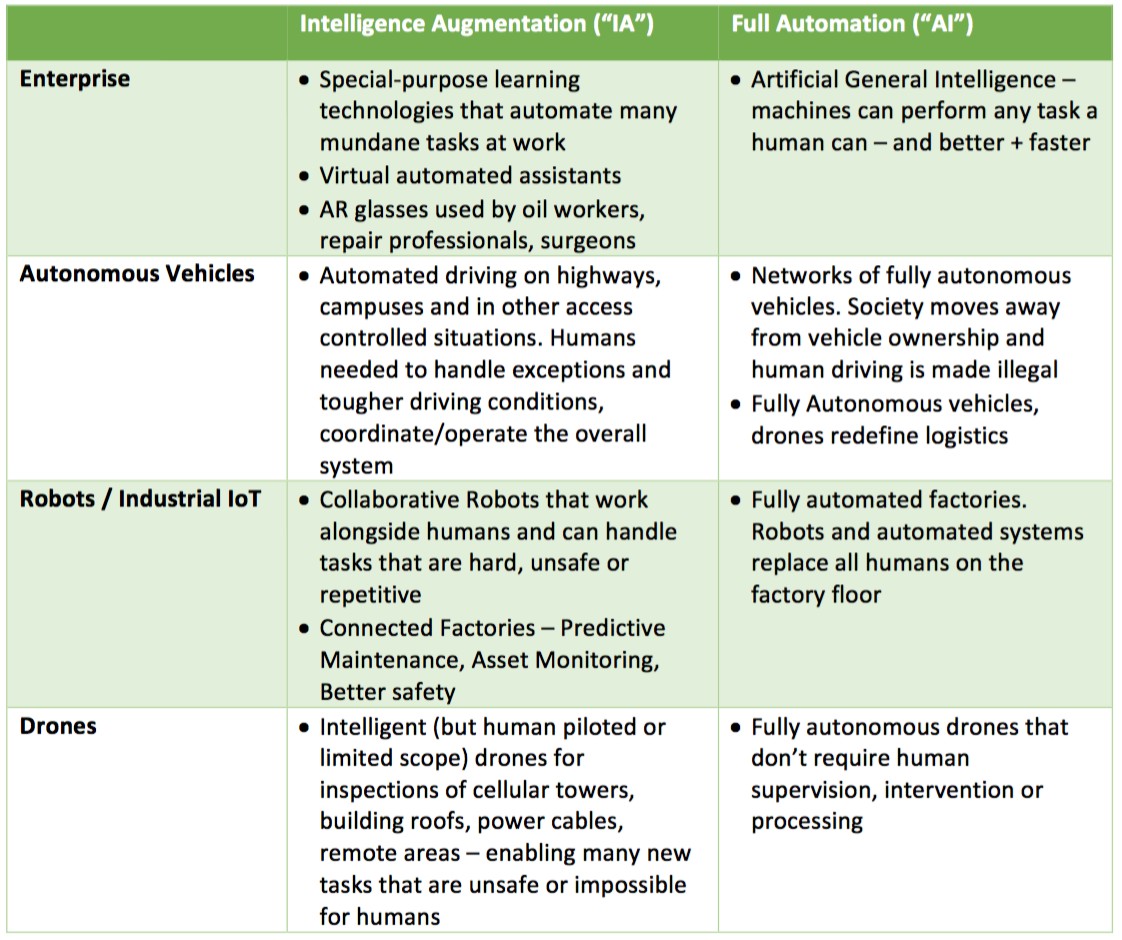
\includegraphics[width=0.9\linewidth]{chapters/introduction/images/ia_vs_ai.png}
	\caption{Comparison between IA and AI\\Source: https://www.cbinsights.com/research/ai-vs-intelligence-augmentation-applications, 02.06.18}
	\label{fig:introduction:ia_vs_ai}
\end{figure}

\section{Architecture}
\autoref{fig:introduction:architecture_overview} shows an overview of the information flow between all participating components of the pipeline developed throughout this thesis, with a combination of both the learning and the prediction architecture. Step 2 (loading the satellite imagery from Microsoft Bing) was required only in the learning phase; that is, for the generation of the training data which were required to train the neural network.

\begin{figure}[H]
    \centering
	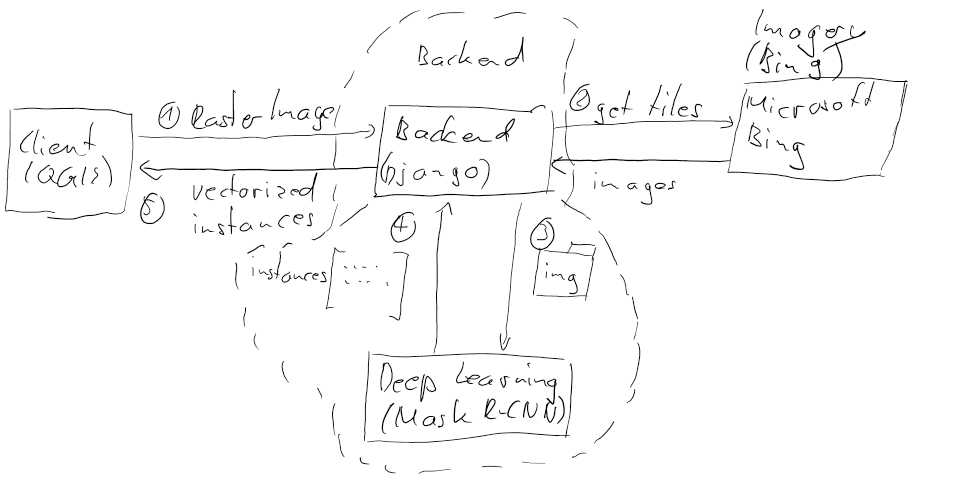
\includegraphics[width=0.9\linewidth]{chapters/introduction/images/overview.png}
	\caption{Architecture overview}
	\label{fig:introduction:architecture_overview}
\end{figure}

\autoref{fig:introduction:learning_phase} shows the data flow during the training of the neural network. For this step, satellite imagery from Microsoft Bing was used, and OpenStreetMap (OSM) data were also mapped. The satellite imagery was downloaded tile-per-tile for a predefined bounding box and zoom-level; at the same time, binary images were created from the OSM data, which represented the ground truth. To simplify this step and make it available to the public, a tool called Airtiler \cite{airtiler} was created and published.

\begin{figure}[H]
    \centering
	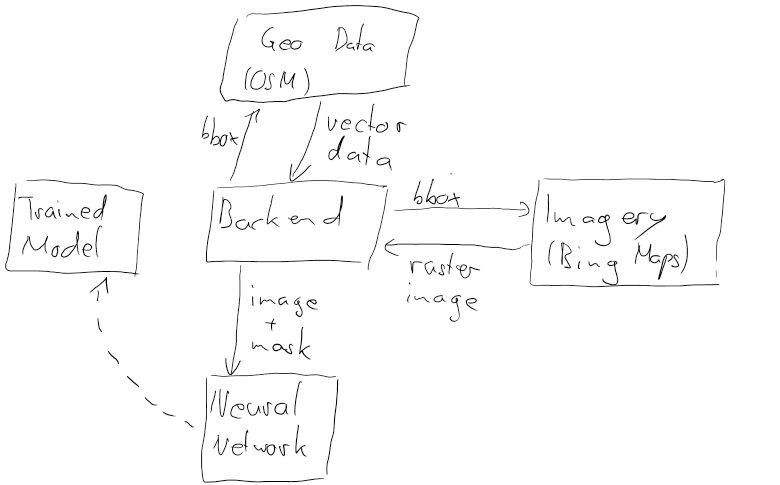
\includegraphics[width=0.9\linewidth]{chapters/introduction/images/learning_phase.png}
	\caption{Learning phase}
	\label{fig:introduction:learning_phase}
\end{figure}

As soon as the training was completed, the prediction could begin. For this thesis, the prediction was split into two phases. \autoref{fig:introduction:prediction_phase1} shows the data flow of phase 1, which passed the current extent as base64 encoded image data as well as the bounding box of the current QGIS extent to the configured backend webserver. The pretrained neural network was then used to predict all instances on the current image. In the next step, the predicted instances were georeferenced using the bounding-box information that was sent to the backend at the beginning of the prediction phase. Finally, the georeferenced instances were sent back to the frontend client, the QGIS plugin. The plugin then visualized the data on a new layer in QGIS.

\begin{figure}[H]
    \centering
	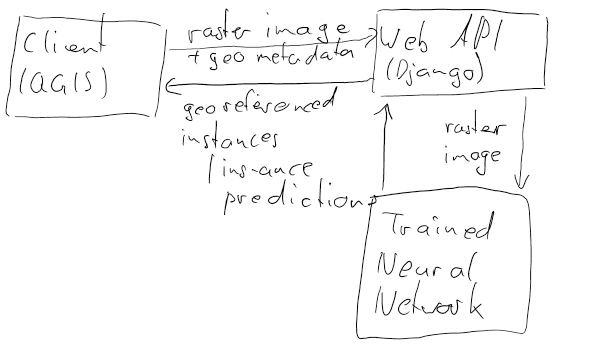
\includegraphics[width=0.9\linewidth]{chapters/introduction/images/inference_phase1.png}
	\caption{Prediction phase 1}
	\label{fig:introduction:prediction_phase1}
\end{figure}

\begin{figure}[H]
    \centering
	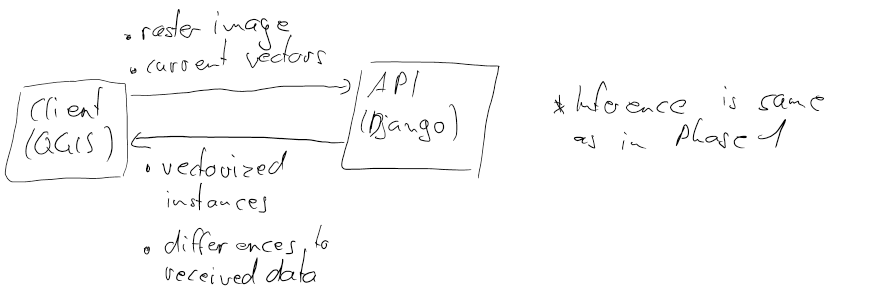
\includegraphics[width=0.9\linewidth]{chapters/introduction/images/inference_phase2.png}
	\caption{Prediction phase 2}
	\label{fig:introduction:prediction_phase2}
\end{figure}

\section{Hardware Requirements}
To train the neural network, a graphics card is required. We used a Nvidia P100 with 12 GB of memory. A Nvidia GTX 750 was insufficient as it had only 2 GB of memory. Additionally, CUDA\footnote{https://developer.nvidia.com/cuda-toolkit (22.06.18)} had to be installed as well as Docker\footnote{https://www.docker.com/ (22.06.18)} and Nvidia-docker\footnote{https://github.com/NVIDIA/nvidia-docker (22.06.18)}. How the docker image can be built and run is described in detail in the readme of the repository\footnote{https://github.com/mnboos/osm-instance-segmentation/blob/master/README.md (22.06.18)}.

\section{User Scenario}
This section describes a user scenario that can be used for demonstration or to instruct the actual end user in how to use the plugin with its corresponding backend. This user scenario requires the plugin to be correctly installed in QGIS. The backend must also be configured correctly in the settings of the plugin, which can be accessed through the dropdown menu of the plugin (\autoref{fig:introduction:plugin_dropdown}). Additionally, the backend was required to be running.
%%
\begin{enumerate}
    \item Start QGIS
    \item 2.	Load the cadastral survey data. This may, for example, be a zip archive containing shape files according to the MOpublic \cite{mopublic}  specification. In this case, the archive can simply be dragged and dropped into QGIS. A dialog will then open, which allows the use to select several layers.
    \item Select the layers containing buildings or other geometries. Typically, according to MOpublic, this layer is named \textit{BB\_BoFlaeche}.
    
    \item Load an imagery layer like Bing maps or Google maps, which can easily be done using the \textit{OpenLayers} QGIS plugin.
    
    \item Open the prediction dialog (\autoref{fig:introduction:prediction_dialog}) by clicking the plugins icon which appears on the \textbf{Manage Layers} toolbar. \autoref{fig:introduction:plugin_icon} shows the plugins icon on the toolbar. \textbf{Alternative:} click the arrow next to the icon and select an option from the dropdown.
    
    \item Select the imagery layer from the dropdown. As shown in \autoref{fig:introduction:prediction_dialog}, a preview of the image that will be sent to the backend is shown at the bottom of the dialog. The appearance of large white areas means that one or more tiles were loaded incorrectly from the corresponding service. In this case, the Refresh button must be clicked at least once, until all white blobs have disappeared.
    
    \item Finally, by clicking the Predict button, the dialog closes and the vectors found are sent to the backend. \textbf{Note:} The backend might take a while to process all the data and hence QGIS might close the network connection; this results in an error if the backend tries to send the response. To solve this problem, the network timeout in the QGIS settings (\autoref{fig:introduction:qgis_timeout}) should be set to a higher value. The connection will then be kept open for a longer period so that the backend can send the response without problems.
\end{enumerate}


\begin{figure}[H]
    \centering
	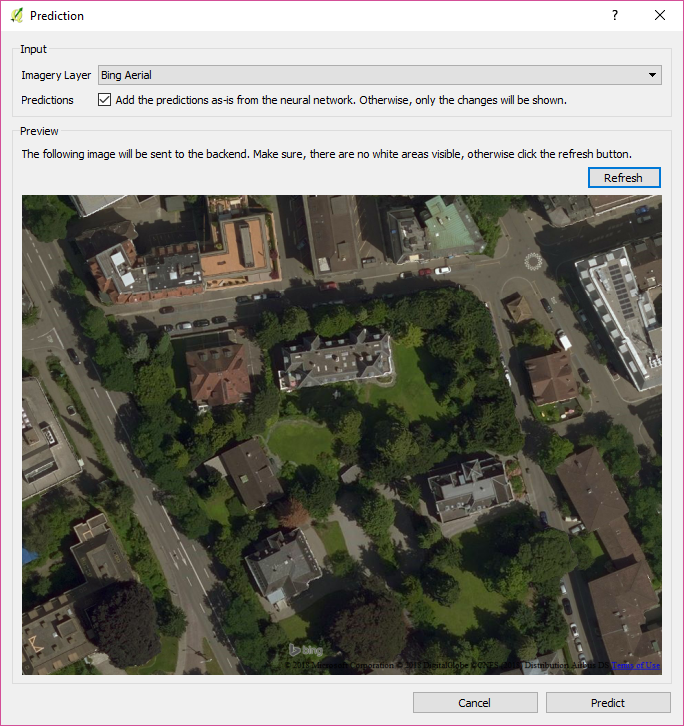
\includegraphics[width=0.8\linewidth]{chapters/introduction/images/prediction_dialog.png}
	\caption{The prediction dialog}
	\label{fig:introduction:prediction_dialog}
\end{figure}

\begin{figure}[H]
    \centering
	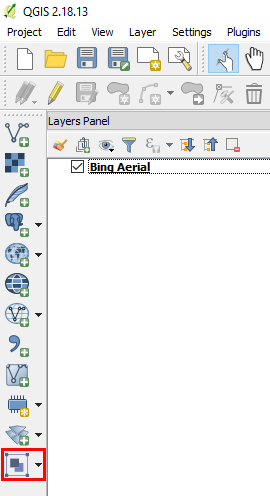
\includegraphics[width=0.5\linewidth]{chapters/introduction/images/plugin_icon.png}
	\caption{The plugins icon on the Manage Layers toolbar}
	\label{fig:introduction:plugin_icon}
\end{figure}

\begin{figure}[H]
    \centering
	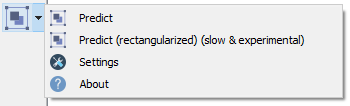
\includegraphics[width=0.5\linewidth]{chapters/introduction/images/plugin_dropdown.png}
	\caption{The plugins dropdown menu}
	\label{fig:introduction:plugin_dropdown}
\end{figure}

\begin{figure}[H]
    \centering
	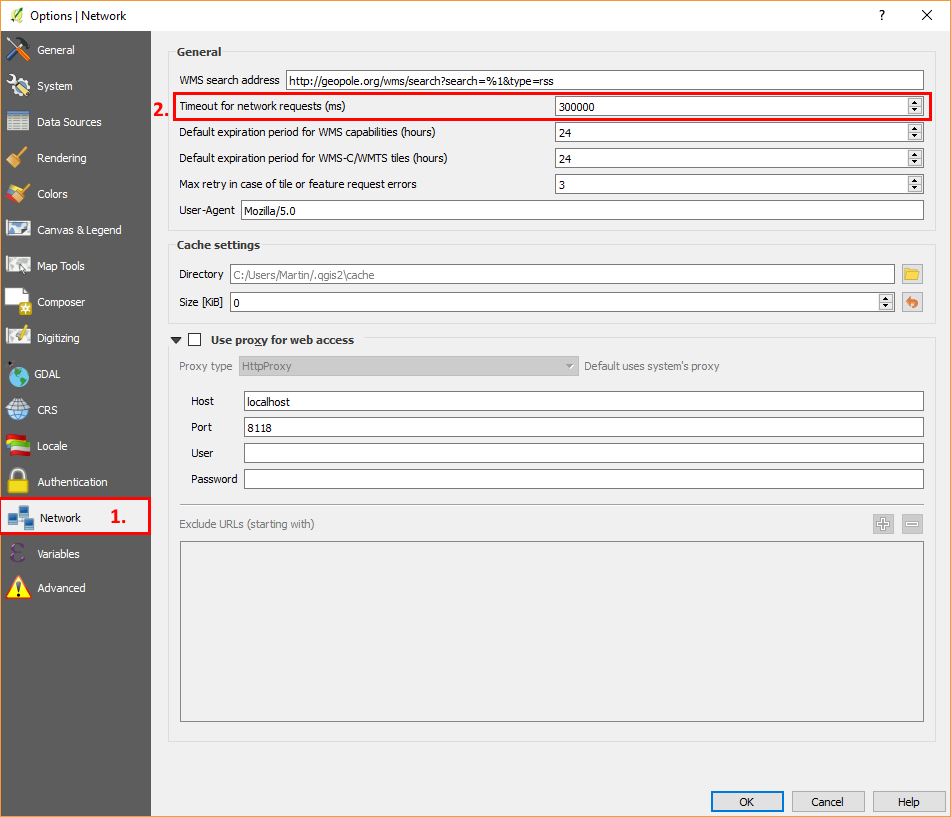
\includegraphics[width=0.8\linewidth]{chapters/introduction/images/qgs_timeout.png}
	\caption{Network timeout configuration in QGIS}
	\label{fig:introduction:qgis_timeout}
\end{figure}

As mentioned earlier, the plugin searches for existing vectors in the loaded layers and sends those that fulfil the QGIS expression  \textbf{\detokenize{"Typ" in ('Gebaeude', 'Strasse_Weg', 'Reben', 'Wasserbecken', 'uebrige_befestigte')}} to the backend. For further details about the communication between the QGIS plugin and the backend, the API specification appear in the appendix of this paper.
